\documentclass{article}

%Page format
\usepackage{pdfpages}
\usepackage{fancyhdr}
\usepackage[margin=1in]{geometry}

%Math packages and custom commands

\usepackage{graphicx}
\usepackage{ textcomp }
\usepackage{algpseudocode}
\usepackage{amsthm}
\usepackage{framed}
\usepackage{hyperref}
\usepackage{tikz}
\usepackage[utf8]{inputenc}
\usepackage[margin=1in]{geometry}
\usepackage{mathtools,amsthm}
\usepackage{enumitem,amssymb}
\newtheoremstyle{case}{}{}{}{}{}{:}{ }{}
\theoremstyle{case}
\newtheorem{case}{Case}
\DeclareMathOperator{\R}{\mathbb{R}}
\DeclareMathOperator{\E}{\mathbb{E}}
\DeclareMathOperator{\Var}{\text{Var}}
\DeclareMathOperator{\Cov}{\text{Cov}}
\newcommand{\bvec}[1]{\mathbf{#1}}
\renewcommand{\P}{\mathbb{P}}
\newcommand{\norm}[2][2]{\| #2\|_{#1}}


\definecolor{shadecolor}{gray}{0.9}

\theoremstyle{definition}
\newtheorem*{answer}{Answer}
\newcommand{\note}[1]{\noindent{[\textbf{NOTE:} #1]}}
\newcommand{\hint}[1]{\noindent{\textit{HINT: #1}}}
\newcommand{\recall}[1]{\noindent{\textit{RECALL: #1}}}
\newcommand{\expect}[1]{\noindent{\fbox{\parbox{0.95 \textwidth}{\textbf{What we expect:} #1}}}}

\newlist{todolist}{itemize}{2}
\setlist[todolist]{label=$\square$}
\usepackage{pifont}
\newcommand{\cmark}{\ding{51}}%
\newcommand{\xmark}{\ding{55}}%
\newcommand{\done}{\rlap{$\square$}{\raisebox{2pt}{\large\hspace{1pt}\cmark}}%
\hspace{-2.5pt}}
\newcommand{\wontfix}{\rlap{$\square$}{\large\hspace{1pt}\xmark}}


\title{\textbf{CS 221: Artificial Intelligence:\\ Principles and Techniques} \\Assignment 3:  Reconstruction}
\date{}

\chead{Assignment 3: Text Reconstruction}
\rhead{\today}
\lfoot{}
\cfoot{CS 221: Artificial Intelligence: Principles and Techniques --- Autumn 2021}
\rfoot{\thepage}
\renewcommand{\headrulewidth}{0.4pt}
\renewcommand{\footrulewidth}{0.4pt}
\pagestyle{fancy}
\setlength{\parindent}{0pt}

\begin{document}

\maketitle

\begin{center}
\begin{tabular}{rl}
SUNet ID: & [your SUNet ID] \\
Name: & [your first and last name] \\
Collaborators: & [list all the people you worked with]
\end{tabular}
\end{center}

\textit{By turning in this assignment, I agree by the Stanford honor code and declare that all of this is my own work.} \\

\begin{figure}[h]
    \centering
    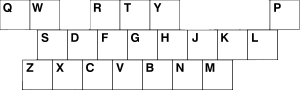
\includegraphics[scale=0.6]{holykeys.png}
\end{figure}


In this homework, we consider two tasks: word segmentation and vowel insertion. Word segmentation often comes up when processing many non-English languages, in which words might not be flanked by spaces on either end, such as written Chinese or long compound German words. Vowel insertion is relevant for languages like Arabic or Hebrew, where modern script eschews notations for vowel sounds and the human reader infers them from context. More generally, this is an instance of a reconstruction problem with a lossy encoding and some context.\newline

We already know how to optimally solve any particular search problem with graph search algorithms such as uniform cost search or A*. Our goal here is modeling --- that is, converting real-world tasks into state-space search problems.

\section*{Setup: $n$-gram language models and uniform-cost search}

Our algorithm will base its segmentation and insertion decisions on the cost of processed text according to a language model. A language model is some function of the processed text that captures its fluency.\newline

A very common language model in NLP is an $n$-gram sequence model. This is a function that, given $n$ consecutive words, provides a cost based on the negative log likelihood that the $n$-th word appears just after the first $n - 1$ words. The cost will always be positive, and lower costs indicate better fluency. As a simple example: In a case where $n=2$ and $c$ is our $n$-gram cost function, $c(\texttt{big}, \texttt{fish})$ would be low, but $c(\texttt{fish}, \texttt{fish})$ would be fairly high.\newline

Furthermore, these costs are additive: For a unigram model $u$ $(n=1)$, the cost assigned to $[w_1,w_2,w_3,w_4]$ is

$$u(w_1)+u(w_2)+u(w_3)+u(w_4).$$

Similarly, for a bigram model $b$ $(n=2)$, the cost is

$$b(w_0,w_1)+b(w_1,w_2)+b(w_2,w_3)+b(w_3,w_4),$$

where $w_0$ is \texttt{-BEGIN-}, a special token that denotes the beginning of the sentence.

We have estimated $u$ and $b$ based on the statistics of $n$-grams in text (\texttt{leo-will.txt}). Note that any words (like ``hello'') not in the corpus are automatically assigned a high cost. This might lead to some unexpected sentences but you do not have to worry about that. \\

\textbf{A note on low-level efficiency and expectations}: This assignment was designed considering input sequences of length no greater than roughly 200, where these sequences can be sequences of characters or of list items, depending on the task. Of course, it's great if programs can tractably manage larger inputs, but it's okay if such inputs can lead to inefficiency due to overwhelming state space growth.\\

You are encouraged to look over the given codebase and how functions like \texttt{cleanLine()} (in \texttt{wordsegUtil.py}) are called by \texttt{grader.py} and \texttt{shell.py} to preprocess lines.
\newpage
\section*{Problem 1: Word Segmentation}

In word segmentation, you are given as input a string of alphabetical characters ($[a-z]$) without whitespace, and your goal is to insert spaces into this string such that the result is the most fluent according to the language model.

\begin{enumerate}
\item[a.]
    Suppose that we have a unigram model $u$ and we are given the string \texttt{breakfastservedinside}. 
    The unigram costs of words are given as $u(\texttt{break})=3$, $u(\texttt{fast})=6$, 
    $u(\texttt{breakfast})=8$, $u(\texttt{served})=8$, $u(\texttt{in})=3$, $u(\texttt{side})=5$, $u(\texttt{inside})=2$. Assume $u(s)=100$ for any other substring $s$ of our string.
    
    Consider the following greedy algorithm:
  begin at the front of the string. Find the
  ending position for the next word that minimizes the
  language model cost. Repeat, beginning at the end of this chosen segment.

    What is the total model cost from running this greedy algorithm on $\texttt{breakfastservedinside}$? 
    Is this greedy search optimal for general inputs? In other words, does it find the lowest-cost segmentation of any input? 
    Explain why or why not in 1-2 sentences.

  \expect{The value of the total model cost and an explanation of why the greedy algorithm is or is not optimal.}
  \begin{shaded}

  \end{shaded}
\newpage
\item[b.]
    Implement an algorithm that, unlike the greedy algorithm, finds the optimal word segmentation of an input character sequence. Your algorithm will consider costs based simply on a unigram cost function. UniformCostSearch (UCS) is implemented for you in $\texttt{util.py}$, and you should make use of it here.

    Before jumping into code, you should think about how to frame this problem as a state-space search problem. How would you represent a state? What are the successors of a state? What are the state transition costs? (You don't need to answer these questions in your writeup.)

    Fill in the member functions of the SegmentationProblem class and the segmentWords function. The argument unigramCost is a function that takes in a single string representing a word and outputs its unigram cost. You can assume that all of the inputs would be in lower case. The function segmentWords should return the segmented sentence with spaces as delimiters, i.e. \texttt{` '.join(words)}.

    For convenience, you can actually run \texttt{python submission.py} to enter a console in which you can type character sequences that will be segmented by your implementation of \texttt{segmentWords}. To request a segmentation, type \texttt{seg mystring} into the prompt. For example:
    \begin{verbatim}
    >> seg thisisnotmybeautifulhouse

    Query (seg): thisisnotmybeautifulhouse

    this is not my beautiful house
    \end{verbatim}

    
    Console commands other than \texttt{seg} --- namely \texttt{ins} and \texttt{both} --- will be used in the upcoming parts of the assignment. Other commands that might help with debugging can be found by typing \texttt{help} at the prompt.
    
  \hint{You are encouraged to refer to \texttt{NumberLineSearchProblem} and \texttt{GridSearchProblem} implemented in \texttt{util.py} for reference. They don't contribute to testing your submitted code but only serve as a guideline for what your code should look like.}
  
  \hint{The actions that are valid for the \texttt{ucs} object can be accessed through \texttt{ucs.actions}.}
  
  \expect{An implementation of the member functions of the \texttt{SegmentationProblem} class and the \texttt{segmentWords} function.}

\end{enumerate}
 \newpage

\section*{Problem 2: Vowel Insertion}

    Now you are given a sequence of English words with their vowels missing (A, E, I, O, and U; never Y). Your task is to place vowels back into these words in a way that maximizes sentence fluency (i.e., that minimizes sentence cost). For this task, you will use a bigram cost function.

    You are also given a mapping \texttt{possibleFills} that maps any vowel-free word to a set of possible reconstructions (complete words). For example, \texttt{possibleFills(`fg')} returns \texttt{set([`fugue', `fog'])}.

\begin{enumerate}
    \item[a.] Consider the following greedy-algorithm: from left to right, repeatedly pick the immediate-best vowel insertion for the current vowel-free word, given the insertion that was chosen for the previous vowel-free word. This algorithm does not take into account future insertions beyond the current word.

    Show that this greedy algorithm is suboptimal, by providing a realistic counter-example using English text. Make any assumptions you'd like about \texttt{possibleFills} and the bigram cost function, but bigram costs must be positive.
    
    In creating this example, lower cost should indicate better fluency. Note that the cost function doesn't need to be explicitly defined. You can just point out the relative cost of different word sequences that are relevant to the example you provide. And your example should be based on a realistic English word sequence -- don't simply use abstract symbols with designated costs. Limit your answers to 4 sentences max to receive full credits.

    \expect{A specific (realistic) example explained within a couple of sentences.}
    
    \begin{shaded}

    \end{shaded}
    
\newpage
    \item[b.]
    Implement an algorithm that finds optimal vowel insertions. Use the UCS subroutines.

    When you've completed your implementation, the function \texttt{insertVowels} should return the reconstructed word sequence as a string with space delimiters, i.e. \texttt{` '.join(filledWords)}. Assume that you have a list of strings as the input, i.e. the sentence has already been split into words for you. Note that the empty string is a valid element of the list.

    The argument \texttt{queryWords} is the input sequence of vowel-free words. Note that the empty string is a valid such word. The argument \texttt{bigramCost} is a function that takes two strings representing two sequential words and provides their bigram score. The special out-of-vocabulary beginning-of-sentence word \texttt{-BEGIN-} is given by \texttt{wordsegUtil.SENTENCE\_BEGIN}. The argument \texttt{possibleFills} is a function that takes a word as a string and returns a \texttt{set} of reconstructions.

    Since we use a limited corpus, some seemingly obvious strings may have no filling, such as \texttt{chclt -> \{\}}, where \texttt{chocolate} is actually a valid filling. Don't worry about these cases.
    
    \note{Only for Problem 2, if some vowel-free word $w$ has no reconstructions according to \texttt{possibleFills}, your implementation should consider $w$ itself as the sole possible reconstruction. Otherwise you should always use one of its possible completions according to \texttt{possibleFills}. This is NOT the case for Problem 3.}

    Use the \texttt{ins} command in the program console to try your implementation. For example:
    \begin{verbatim}
    >> ins thts m n th crnr

    Query (ins): thts m n th crnr

    thats me in the corner
    \end{verbatim}
    The console strips away any vowels you do insert, so you can actually type in plain English and the vowel-free query will be issued to your program. This also means that you can use a single vowel letter as a means to place an empty string in the sequence. For example:
    \begin{verbatim}
    >> ins its a beautiful day in the neighborhood

        Query (ins): ts  btfl dy n th nghbrhd

        its a beautiful day in the neighborhood
    \end{verbatim}
    \expect{An implementation of the member functions of the \texttt{VowelInsertionProblem} class and the \texttt{insertVowels} function.}

\end{enumerate}

\newpage

\section*{Problem 3: Putting it Together}

We'll now see that it's possible to solve both of these tasks at once. This time, you are given a whitespace-free and vowel-free string of alphabetical characters. Your goal is to insert spaces and vowels into this string such that the result is as fluent as possible. As in the previous task, costs are based on a bigram cost function.

\begin{enumerate}
    \item[a.]
    Consider a search problem for finding the optimal space and vowel insertions. Formalize the problem as a search problem: What are the states, actions, costs, initial state, and end test? Try to find a minimal representation of the states.
    
    \expect{A formal definition of the search problem with definitions for the states, actions, costs, initial state, and end test.}
    \begin{shaded}

    \end{shaded}
\newpage
    \item[b.]
	Implement an algorithm that finds the optimal space and vowel insertions. Use the UCS subroutines.

When you've completed your implementation, the function \texttt{segmentAndInsert} should return a segmented and reconstructed word sequence as a string with space delimiters, i.e. \texttt{` '.join(filledWords)}.

The argument \texttt{query} is the input string of space- and vowel-free words. The argument \texttt{bigramCost} is a function that takes two strings representing two sequential words and provides their bigram score. The special out-of-vocabulary beginning-of-sentence word \texttt{-BEGIN-} is given by \texttt{wordsegUtil.SENTENCE\_BEGIN}. The argument \texttt{possibleFills} is a function that takes a word as a string and returns a \texttt{set} of reconstructions.

\note{In problem 2, a vowel-free word could, under certain circumstances, be considered a valid reconstruction of itself. However, for this problem, in your output, you should only include words that are the reconstruction of some vowel-free word according to \texttt{possibleFills}. Additionally, you should not include words containing only vowels such as \texttt{a} or \texttt{i} or out of vocabulary words; all words should include at least one consonant from the input string and a solution is guaranteed. Additionally, aim to use a minimal state representation for full credit.}

Use the command \texttt{both} in the program console to try your implementation. For example:
    \begin{verbatim}
    >> both mgnllthppl

        Query (both): mgnllthppl

        imagine all the people
    \end{verbatim}
  \expect{An implementation of the member functions of the \texttt{JointSegmentationInsertionProblem} class and the \texttt{segmentAndInsert} function.}
  

 
\end{enumerate}

\newpage
\section*{Problem 4: Failure Modes and Transparency}
Now that you have a working reconstruction algorithm, let’s try reconstructing a few examples. Take each of the below phrases and pass them to the both command from the program console.
\begin{itemize}
\item Example 1: “yrhnrshwllgrcslyccptthffr” (original: “your honor she will graciously accept the affair”)
\item Example 2: “wlcmtthhttkzn” (original: “welcome to the hot take zone”)
\item Example 3: “grlwllnrflprrghtnw” (original: “girl we all in our flop era right now”)
\end{itemize}

\begin{enumerate}
    \item[a.]
    First, indicate which examples were reconstructed correctly versus incorrectly. Recall that the system chooses outputs based on a bigram cost function [4], which is roughly low if a bigram occurred in Leo Tolstoy's \textit{War and Peace} and William Shakespeare's \textit{Romeo and Juliet}, and high if it didn't (the details don't matter for this problem). Then, explain what about the training data may have led to this behavior.
    
    \expect{1-2 sentences listing whether each example was correctly or incorrectly reconstructed and a brief explanation \underline{with justification} as to what about the training data may have led to this result.}
    \begin{shaded}
    \end{shaded}
    
    \newpage
    \item[b.]
    Your system, like all systems, has limitations and potential points of failure. As a responsible AI practitioner, it’s important for you to recognize and communicate these limitations to users of the systems you build. Imagine that you are deploying your search algorithm from this assignment to real users on mobile phones.
    Write a \textbf{transparency statement} for your system,
    which communicates to users the conditions under which the system should be
    expected to work and when it might not work.
    
    \expect{2-4 sentences explaining the potential failure modes of
    your system. Be sure to acknowledge the limitations that your system has
    and who should know about these limitations (i.e., who are the affected
    parties?).}
    \begin{shaded}
    \end{shaded}
    
    \newpage
    \item[c.]
    Given the limitations found in part (a) and described in your transparency statement from (b), how could you improve your system?
    
    \expect{2-4 sentences proposing a change to the cost function, how you would implement it,
    and why it would address the limitations you identified above.}
    \begin{shaded}
    \end{shaded}
\end{enumerate}

% \newpage
% \section*{Problem 5: A* Karel!}
% We'll now see a basic application of A* search in the context of everyone's favorite robot, Karel! In our context, Karel has a cookie craving and is trying to reach the cell with the cookie in the fewest number of commands while not entering the lava lake. Karel is hungry and aims to use A* search to optimize the cookie search and needs your help. Note that Karel can only use the following commands: \texttt{turnLeft()}, \texttt{turnRight()}, \texttt{moveForward()}. Karel can finish one command in 1 time step in white cells, but needs 10 time steps to finish one command in the swamp (dark green cells).

% \begin{figure}[h]
%     \centering
%     
\includegraphics[scale=0.6]{astar_search.png}
% \end{figure}


% \begin{enumerate}
%     \item[a.]
%      The bottom left cell in the grid shown above is $(0, 0)$ in the Cartesian plane. Karel is currently at cell $(1, 0)$, is facing East, and wants to reach the cell containing the cookie (facing any direction). We can define $T^{*}(a, b, d)$ to be the minimum number of commands Karel needs to reach the cookie starting from cell $(a, b)$ and initially facing direction $d$. Assume for this part that Karel has an admissible heuristic $h(a, b, d)$. What can we say about how $h(1, 0, East)$ compares to $T^{*}(1, 0, East)$?


%   \expect{A mathematical expression relating $h(1, 0, East)$ to $T^*(1,0, East)$ along with a brief justification.}

%   \begin{shaded}

%   \end{shaded}
% \newpage
%   \item[b.]
%   How would we define an admissible heuristic $h(a, b, d)$ for Karel as described in part a)? In particular, how could we relax Karel's search problem to define a different cost metric, which is always optimistic when used as a heuristic in the original (non-relaxed) setting? Explain why the cost metric you define is always optimistic. Note that Karel always knows the final (cell) position of the cookie.
  
%   Here "optimistic" describes the property of a heuristic, and oftentimes, we choose our heuristic for a search problem to be the cost metric for a relaxed version of the search problem. For this question, we want you to come up with a relaxed version of Karel's search problem, and define its cost metric, which is used as the heuristic for the original problem. You need to explain why this heuristic is always optimistic.
  
%   \expect{A description of a relaxed search problem and a definition of a different cost metric with a justification for why it is always optimistic. The cost metric should be concrete (i.e., explain exactly how the cost is computed in the relaxed setting).}

%   \begin{shaded}

%   \end{shaded}
% \end{enumerate}

\newpage
\section*{Submission}

Submission is done on Gradescope. \\

\textbf{Written:} When submitting the written parts, make sure to select \textbf{all} the pages that contain part of your answer for that problem, or else you will not get credit.
To double check after submission, you can click on each problem link on the right side and it should show the pages that are selected for that problem. \\

\textbf{Programming:} After you submit, the autograder will take a few minutes to run. Check back after it runs to make sure that your submission succeeded. If your autograder crashes, you will receive a 0 on the programming part of the assignment. Note: the only file to be submitted to Gradescope is $\texttt{submission.py}$.\\

More details can be found in the Submission section on the course website.

\newpage
\begin{thebibliography}{9}
\bibitem{reference}
In German, Windschutzscheibenwischer is "windshield wiper." Broken into parts: wind = wind; schutz = block / protection; scheiben = panes; wischer = wiper.
\bibitem{reference}
See \href{https://en.wikipedia.org/wiki/Abjad}{https://en.wikipedia.org/wiki/Abjad}
\bibitem{reference}
This model works under the assumption that text roughly satisfies the \href{https://en.wikipedia.org/wiki/Markov_property}{Markov property}.
\bibitem{reference}
Modulo edge cases, the $n$-gram model score in this assignment is
  given by $\ell(w_1, \ldots, w_n) = -\log p(w_n \mid w_1, \ldots,
  w_{n-1})$.  Here, $p(\cdot)$ is an estimate of the conditional
  probability distribution over words given the sequence of previous
  $n-1$ words. This estimate is based on word frequencies
  in Leo Tolstoy's \textit{War and Peace} and William
  Shakespeare's \textit{Romeo and Juliet}.
\bibitem{reference}
Solutions that use UCS ought to exhibit fairly fast execution time for this problem, so using A* here is unnecessary.
\bibitem{reference}
This mapping was also obtained by reading Tolstoy and Shakespeare and removing vowels.
\end{thebibliography}

\end{document}